\chapter{Introduction}
\label{Introduction}

\section{Recent Trends in Statistics}
\label{RecentTrendsinStatistics}
Data-storage and data-capture devices have consistently become both cheaper and more powerful allowing enormous amounts of data to be collected. The computational power of computers needed to sift through this data has also increased exponentially\footnote{Increases in computational power have so far grown according to Moore's Law (1965)~\cite{Moore1965} which roughly states that the number of transistors in integrated circuits doubles every 2 years.}. With enormous pools of specialist commercial and scientific data that have since been amassed, there is great potential for knowledge discovery from these databases. Prime examples include data gathered from supermarket loyalty cards, the Human Genome Project and the Internet. The ability to understanding consumer shopping habits, predispositions to genetic disorders and helping people find information on the Internet holds great commercial value.\\

Applied Statisticians have made great strides in this area tackling data-related problems ranging from Bioinformatics to Optical Character Recognition and have done so by marrying the power of computers with ideas from Statistics. In doing so, they have greatly increased the range of problems that Statistics can be used to tackle. \\

Though much progress has been made in the field of Pattern Recognition, it is often difficult for non-specialist users to apply such techniques to real-world datasets as academic work is often too specialized for easy use and proprietary software often written for profit. As a result, such ideas cannot have reached their full potential. There has however been movement in recent years towards providing widely accessible open-source software\footnote{R~\cite{R} is a free software environment for statistical computing which gathers open-source implementations of an extensive collection of statistical and graphical techniques. It has become a defacto standard for developers of statistical software due to its highly extensible nature and its ease of use.} to address these issues via a program called R. With vast improvements in computational power and a growing collection of easily extensible statistical programs, it has become worthwhile to revisit problems that were once considered too difficult. 

%The computational power of computers has increased by an order of a thousand since the early 1980's till now
\section{Aim of this Thesis}
\label{AimofthisThesis}
The Classification Tree is a widely used classifier introduced in its current form by Breiman \emph{et al}~\cite{cart84-2} in the 1980's. Like all other classifiers, a Classification Tree is simply a model that makes predictions of the class of previously unobserved observations as illustrated in Figure~\ref{fig_typical_classifier}. \\
\begin{figure}
\centering
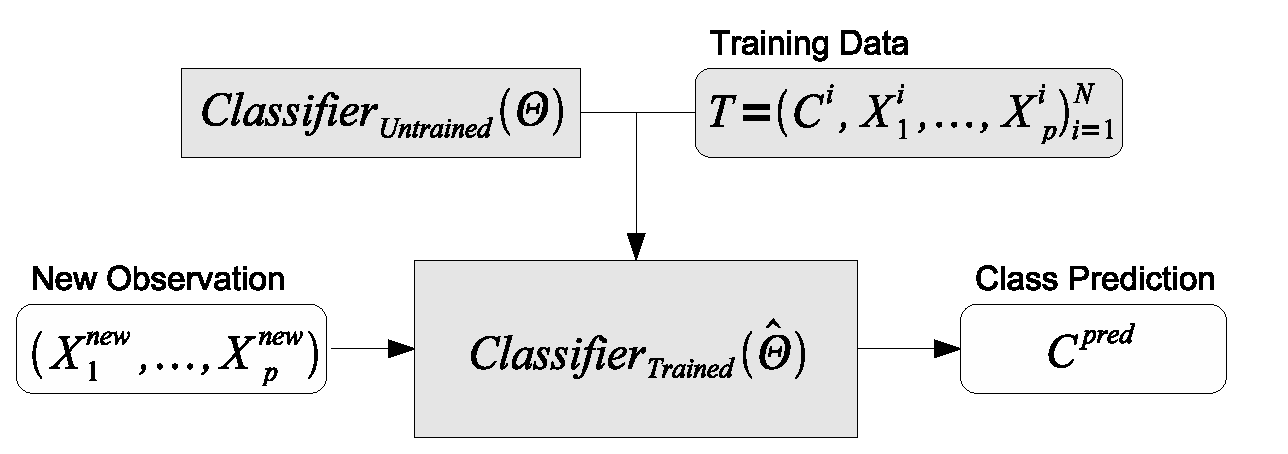
\includegraphics[width=1\textwidth]{fig_typical_classifier.eps}
\caption{A classification model makes predictions of the class of observations by viewing attributes $\left(X_1^{new},\ldots,X_p^{new}\right)$ measured from it. A classifier must firstly be trained to some data $\mathcal{T}$ to find parameters that allow it to model observations from such a population. A trained classifier can therefore make informed predictions of the class $C^{pred}$ of previously unobserved observations.}
\label{fig_typical_classifier}
\end{figure}

The main strength of a Classification Tree is the simplicity with which it makes these predictions. One follows a flow diagram (called a tree) performing a series of predefined tests which eventually leads to a prediction. It is an interpretable and opaque process which appeals to many practitioners.\\

Though there are many possible applications of this idea, Classification and Regression Trees (CART trees) proposed by Breiman \emph{et al} are the most widely used form. It mainly focuses on using dichotomous tests of the form $X_i<c$ (axis-parallel splits) over continuous attributes for two main reasons, 
\begin{itemize}
\item[-] axis-parallel splits are interpretable and 
\item[-] more importantly they are easy to implement even for large datasets.
\end{itemize}
Though CART trees are considered to be interpretable relative to other classifiers, its interpretability diminishes with the size of a tree (the number of tests it uses) so it is desirable to find ways of obtaining smaller trees. One way of achieving this is to consider more general tests, say of the form $\sum_i a_iX_i<c$ (summing over continuous attributes $X_i$). Such tests will be called oblique splits\footnote{Tests of the form $\sum_i a_iX_i<c$ have been known by many names as many researchers have worked on incorporating them into trees. Other names include Linear Machines, Linear-Combination Tests, Multivariate Tests and Oblique Splits.}.\\

Though many attempts have been made at growing\footnote{Trees are said to be grown as well as trained to training data.} oblique trees (trees grown by considering oblique splits over continuous attributes), none have caught on; axis-parallel trees (those that consider axis-parallel splits over continuous attributes) are still widely used. This thesis aims to identify and address potential reasons for this so that oblique trees may be better utilized.

\section{Organization of this Thesis}
\label{OrganizationofthisThesis}
This thesis is organized as follows. Chapter~\ref{Introduction} contains a brief overview of recent developments in Information Technology and its relation to modern Applied Statistics. A description of the aim of this thesis follows with an overview of the thesis. \\

Chapter~\ref{Background} identifies possible reasons as to why existing approaches to growing oblique trees are shunned. Starting with a recap of the basic idea of a Classification Tree, a discussion on how oblique splits might be used to improve tree interpretability is given. A summary of likely reasons for their lack of use follows. \\

Chapter~\ref{ExistingWork} surveys existing approaches to growing oblique trees. Existing work is separated into the two philosophies by which they find oblique splits to provide a clearer understanding of the material as well as its progression. \\

Chapter~\ref{ObliqueSplitsviaProbabilisticModels} presents a new approach to finding oblique splits with real-life examples. A heuristic argument further backing the proposed approach is follows. \\

!!!!!!!!!!!!!!!!!!!!!
Chapter~\ref{InterpretableObliqueTrees} present methods of obtaining interpretable oblique trees. Methods are broadly separated into two groups, those applied during tree growth and those applied post-tree growth.\\

An in-depth analysis of techniques presented in this thesis are given in Chapter~\ref{AdditionalPoints}. It explores its weaknesses and limitations and highlights situations where it performs well.\\

Chapter~\ref{ConcludingRemarks} concludes with final remarks for work in this thesis.